
LLVM是一个庞大的软件,由数百个组件紧密协作,其不断增加的运行时间正慢慢成为一个问题。这影响了许多对编译时间敏感的用例,例如:即时(JIT)编译器。为了系统地诊断这个问题,LLVM提供了一些有用的工具来分析执行时间。

运行时长分析一直是软件开发中的一个重要话题。通过从单个软件组件中收集运行时间,我们可以更容易地发现性能瓶颈。本节中,我们将了解LLVM提供的两个工具:\texttt{Timer}类和\texttt{TimeTraceScope}类。我们先从\texttt{Timer}类开始。

\subsubsubsection{11.4.1\hspace{0.2cm}Timer类}

\texttt{Timer}类,顾名思义,可以度量代码区域的执行时间。下面是一个例子:

\begin{lstlisting}[style=styleCXX]
#include "llvm/Support/Timer.h"
…
Timer T("MyTimer", "A simple timer");
T.startTimer();
// Do some time-consuming works…
T.stopTimer();
\end{lstlisting}

前面的代码中,\texttt{Timer}实例\texttt{T}测量在该区域中花费的时间,该区域使用\texttt{startTimer}和\texttt{stopTimer}方法进行耗时测量。

现在我们已经收集了耗时数据,让我们试着将其打印出来。下面是一个例子:

\begin{lstlisting}[style=styleCXX]
Timer T(…);
…
TimeRecord TR = T.getTotalTime();
TR.print(TR, errs());
\end{lstlisting}

在前面的代码中,\texttt{TimeRecord}实例封装了由\texttt{Timer}类收集的数据。然后,使用\texttt{TimeRecord::print}将其打印到流中——在本例中是\texttt{errors()}流。此外,指定了另一个\texttt{TimeRecord}实例——通过\texttt{print}的第一个参数——作为总耗时。来看看这段代码的输出:

\begin{tcblisting}{commandshell={}}
===---------------------------------------------------------===
                Miscellaneous Ungrouped Timers
===---------------------------------------------------------===
---User Time--- --User+System-- ---Wall Time--- ---Name ---
 0.0002 (100.0%) 0.0002 (100.0%) 0.0002 (100.0%) A simple timer
 0.0002 (100.0%) 0.0002 (100.0%) 0.0002 (100.0%)   Total
 0.0002 (100.0%) 0.0002 (100.0%) 0.0002 (100.0%)
\end{tcblisting}

前面的输出中,第一行显示了从前面的\texttt{Timer}实例收集的\texttt{TimeRecord}实例,而第二行显示了总时间——\texttt{TimeRecord::print}的第一个参数。

现在,我们知道如何打印由单个\texttt{Timer}实例收集的计时数据,但是如果有多个计时器呢?LLVM为\texttt{Timer}类提供了另一个支持工具:\texttt{TimerGroup}类。下面是使用\texttt{TimerGroup}类的例子:

\begin{lstlisting}[style=styleCXX]
TimerGroup TG("MyTimerGroup", "My collection of timers");

Timer T("MyTimer", "A simple timer", TG);
T.startTimer();
// Do some time-consuming works…
T.stopTimer();

Timer T2("MyTimer2", "Yet another simple timer", TG);
T2.startTimer();
// Do some time-consuming works…
T2.stopTimer();

TG.print(errs());
\end{lstlisting}

在前面的代码中,我们声明了一个\texttt{TimerGroup}实例\texttt{TG},并将它用作创建\texttt{Timer}实例的第三个构造函数参数。最后,使用\texttt{TimerGroup::print}进行打印。下面是这段代码的输出:

\begin{tcblisting}{commandshell={}}
===---------------------------------------------------------===
                    My collection of timers
===---------------------------------------------------------===
Total Execution Time: 0.0004 seconds (0.0004 wall clock)
  ---User Time--- --User+System-- ---Wall Time--- ---Name ---
  0.0002 ( 62.8%) 0.0002 ( 62.8%) 0.0002 ( 62.8%) A simple timer
  0.0001 ( 37.2%) 0.0001 ( 37.2%) 0.0001 ( 37.2%) Yet another simple timer
  0.0004 (100.0%) 0.0004 (100.0%) 0.0004 (100.0%) Total
\end{tcblisting}

输出中的每一行(最后一行除外)都是该组中\texttt{Timer}的\texttt{TimeRecord}实例。

目前为止,我们一直使用\texttt{Timer::startTimer}和\texttt{Timer::stopTimer}来切换计时器。为了在不手动调用这两个方法的情况下,更容易地测量代码块内的时间间隔(即用大括号\texttt{\{\}}括起来的区域),LLVM提供了另一个工具,可以在进入代码块时自动启动计时器,并在退出时关闭计时器。让我们看看如何使用\texttt{TimeRegion}类:

\begin{lstlisting}[style=styleCXX]
TimerGroup TG("MyTimerGroup", "My collection of timers");
{
	Timer T("MyTimer", "A simple timer", TG);
	TimeRegion TR(T);
	// Do some time-consuming works…
} {
	Timer T("MyTimer2", "Yet another simple timer", TG);
	TimeRegion TR(T);
	// Do some time-consuming works…
}

TG.print(errs());
\end{lstlisting}


这里,我们没有调用\texttt{startTimer}/\texttt{stopTimer},而是将要测量的代码放入单独的代码块中,并使用\texttt{TimeRegion}变量来自动切换计时器,这段代码将输出与前一个示例相同的内容。\texttt{TimeRegion}的帮助下,可以有一个更简洁的语法,并避免忘记关闭计时器导致的错误。

现在,我们已经了解了如何使用\texttt{Timer},及其支持的实用程序来测量某个代码区域的执行时间。下一节中,我们将了解一种更高级的时间测量方式(可以捕获程序的层次结构)。


\subsubsubsection{11.4.2\hspace{0.2cm}收集时间轨迹}

前一节中,我们了解了如何使用\texttt{Timer}来收集一段代码区域的执行时间。虽然这提供了编译器运行时性能的描述,但有时我们需要一个更结构化的时间配置文件,以便完全理解系统问题。

\texttt{TimeTraceScope}是LLVM提供的一个类,用于执行全局范围的时间分析。它的用法非常简单:类似于在前一节中看到的\texttt{TimeRegion},\texttt{TimeTraceScope}实例在进入和退出代码块时自动打开和关闭时间分析器。下面是一个例子:

\begin{lstlisting}[style=styleCXX]
TimeTraceScope OuterTimeScope("TheOuterScope");
for (int i = 0; i < 50; ++i) {
	{
		TimeTraceScope InnerTimeScope("TheInnerScope");
		foo();
	}
	bar();
}
\end{lstlisting}

前面的代码片段中,我们创建了两个\texttt{TimeTraceScope}实例:\texttt{OuterTimeScope}和\texttt{InnerTimeScope}。它们分别尝试分析整个区域的执行时间和\texttt{foo}函数耗费的时间。

通常,我们会使用\texttt{Timer},而不是\texttt{TimeTraceScope},虽然它只能提供从每个计时器收集到的累计持续时间。然而,在这种情况下,我们更感兴趣的是代码的不同部分如何在时间轴上分配自己的时间,例如:\texttt{foo}函数是否每次循环迭代都耗费相同的时间?如果不是,那么哪个迭代会比其他迭代耗费更多的时间?

要查看结果,需要在运行Pass时向\texttt{opt}命令添加额外的命令行选项(假设在Pass中使用\texttt{TimeTraceScope})。下面是一个例子:

\begin{tcblisting}{commandshell={}}
$ opt –passes="…" -time-trace -time-trace-file=my_trace.json …
\end{tcblisting}

\texttt{-time-trace}标志要求\texttt{opt}将\texttt{TimeTraceScope}收集的所有轨迹信息,导出到\texttt{-time-trace-file}选项指定的文件中。

运行此命令后,将得到一个新文件\texttt{my\_trace.jso}n。这个文件的内容不是人能看的,但想看也有办法。可以使用\textbf{Chrome}网络浏览器将其可视化。以下是实现这一目标的步骤:

\begin{enumerate}
\item 打开Chrome浏览器,在\textbf{URL(Uniform Resource Locator)}栏中输入\texttt{Chrome://tracing}。会看到这样一个界面:

\hspace*{\fill} \\ %插入空行
\begin{center}
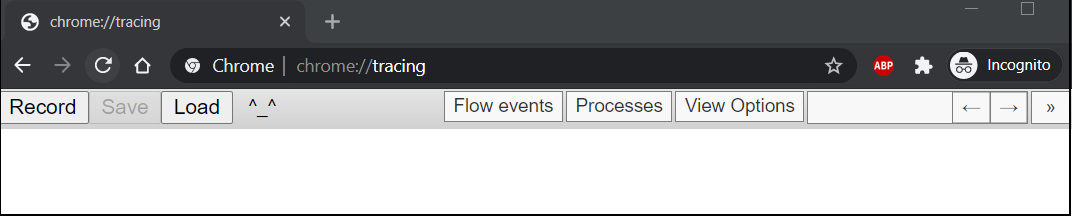
\includegraphics[width=0.9\textwidth]{content/3/chapter11/images/3.png}\\
图11.3 - Chrome中的跟踪可视化工具
\end{center}

\item 点击左上角的\textbf{Load}按钮,选择\texttt{my\_trace.json}文件。会看到这样一个页面:

\hspace*{\fill} \\ %插入空行
\begin{center}
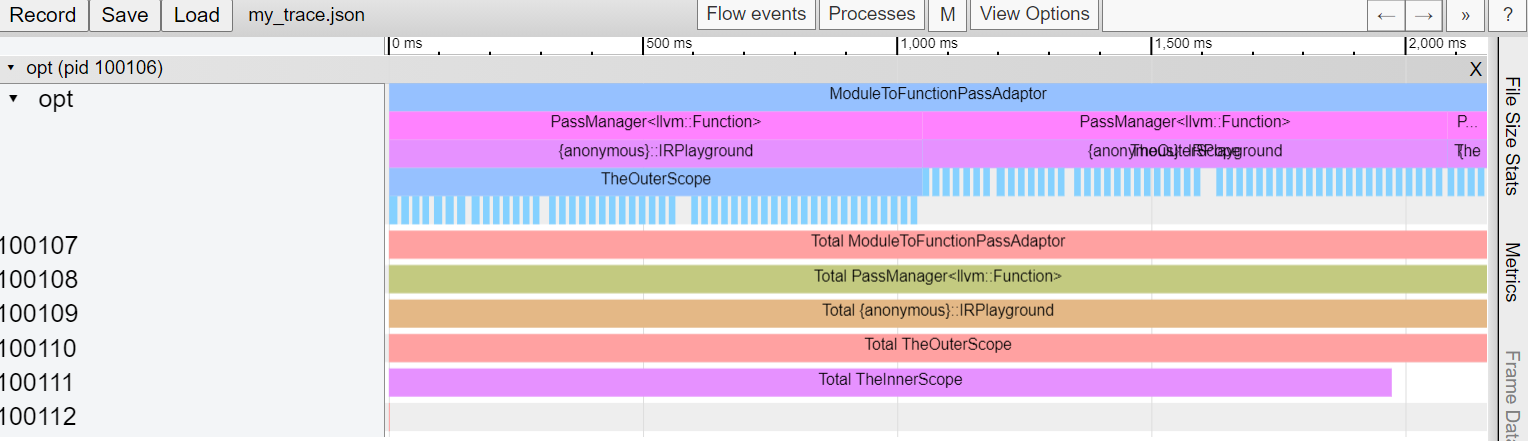
\includegraphics[width=0.9\textwidth]{content/3/chapter11/images/4.png}\\
图11.4 - 打开\texttt{my\_trace.json}后的视图
\end{center}

每个色块代表由\texttt{TimeTraceScope}实例收集的耗时情况。

\item 来仔细看看:请按数字键3切换到缩放模式。之后,应该能够通过点击和拖动鼠标向上或向下,进行放大或缩小的操作。同时,可以使用方向键向左或向右滚动时间轴。这是我们放大后时间线的一部分:

\hspace*{\fill} \\ %插入空行
\begin{center}
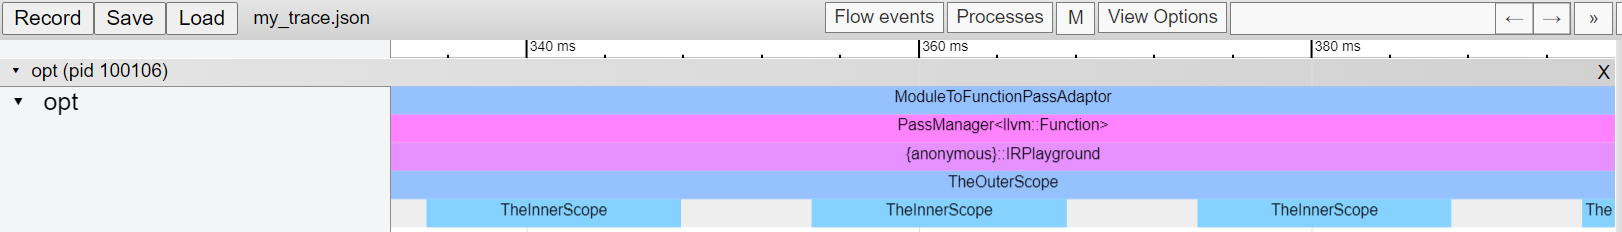
\includegraphics[width=0.9\textwidth]{content/3/chapter11/images/5.png}\\
图11.5 - 时间线的一部分
\end{center}

如图11.5所示,有几个层叠加在一起。这个布局反映了不同的\texttt{TimeTraceScope}实例是如何在\texttt{opt}(和我们的Pass)中执行的,例如:我们的\texttt{TimeTraceScope}实例名为\texttt{TheOuterScope},它堆叠在多个\texttt{TheInnerScope}块之上。每个\texttt{TheInnerScope}块代表了,的\texttt{foo}函数在每次循环迭代中耗费的时间。

\item 我们可以通过点击一个块来进一步检查它的属性,例如:如果点击其中一个\texttt{TheInnerScope}块,它的计时属性将显示在屏幕的下半部分:

\hspace*{\fill} \\ %插入空行
\begin{center}
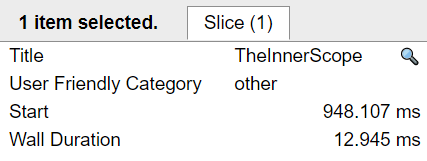
\includegraphics[width=0.5\textwidth]{content/3/chapter11/images/6.png}\\
图11.6 - 耗时块的详细信息
\end{center}

这将为我们提供耗时和开始时间等信息。

\end{enumerate}

通过这种可视化,可以将计时信息与编译器的结构结合起来,从而帮助我们更快地发现性能瓶颈。

除了\texttt{opt}之外,\texttt{clang}还可以生成相同的跟踪JSON文件(请添加\texttt{-ftime-trace})。下面是一个例子:

\begin{tcblisting}{commandshell={}}
$ clang -O3 -ftime-trace -c foo.c
\end{tcblisting}

这将生成与输入文件同名的JSON跟踪文件(本例中是\texttt{foo.json}),可以用我们刚学过的方法把它可视化。

本节中,我们了解了一些从LLVM收集统计信息的有用技能。\texttt{Statistic}类可以用作整数计数器,来记录在优化过程中发生的事件的数量。另一方面,优化注释可以让我们了解优化Pass中的一些决策过程,使编译器开发人员更容易判断错过的优化机会。使用\texttt{Timer}和\texttt{TimeTraceScope},开发人员可以以一种更易于管理的方式监控LLVM的执行时间,并有信心地优化编译速度。这些技术可以提高LLVM开发人员在创造新发明,或解决具有挑战性的问题时的效率。

本章的下一节中,我们将蓼莪及如何使用LLVM提供的工具,以一种高效的方式编写错误处理的代码。





